\begin{align}
 P ( a \textless x \textless b ) =  F(b) - F(a) \end{align}
We want, 
 \begin{align}
S&= P ( {\dfrac{1}{4}}  \textless  X \textless  1)\\
S&= F(1) - F(\dfrac{1}{4})  \\
S&= \dfrac{3}{4} - \dfrac{1^2}{4^2} \\
S&= \dfrac{11}{16}
\end{align}
Hence, P( ${\frac{1}{4}}$ $ \textless $ X $\textless $ 1) is equal to $\frac{11}{16}$

\begin{figure}[!ht]
\centering
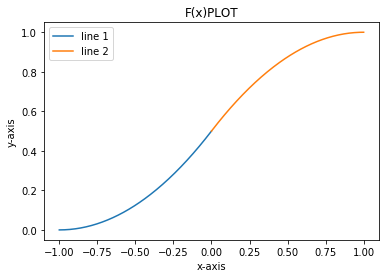
\includegraphics[width=0.5\textwidth]{solutions/ec/54/codes/graph.png}
\label{ec54:fig:graph.png}
\end{figure}


